\documentclass{article}
\usepackage{graphicx} % Required for inserting images

\documentclass[a4paper, 12pt]{article}%тип документа

%отступы
\usepackage[left=2cm,right=2cm,top=2cm,bottom=3cm,bindingoffset=0cm]{geometry}
\usepackage[pdftex]{lscape}
%Русский язык
\usepackage[T2A]{fontenc} %кодировка
\usepackage[utf8]{inputenc} %кодировка исходного кода
\usepackage[english,russian]{babel} %локализация и переносы
\usepackage{multirow}
%Вставка картинок
\usepackage{wrapfig}
\usepackage{graphicx}
\graphicspath{{Images/}}
\DeclareGraphicsExtensions{.pdf,.png,.jpg}

%Математика
\usepackage{amsmath, amsfonts, amssymb, amsthm, mathtools}

%Заголовокhttps://www.overleaf.com/project/6507f5a4176b25bf05722230

\begin{document}

\begin{titlepage}
	\begin{center}
		{\large МОСКОВСКИЙ ФИЗИКО-ТЕХНИЧЕСКИЙ ИНСТИТУТ (НАЦИОНАЛЬНЫЙ ИССЛЕДОВАТЕЛЬСКИЙ УНИВЕРСИТЕТ)}
	\end{center}
	\begin{center}
		{\large Физтех-школа биологической и медицинской физики}
	\end{center}
	
	
	\vspace{4.5cm}
	{\huge
		\begin{center}
			{\bf Отчёт о выполнении лабораторной работы}\\
			Спектрофлуориметрический анализ
		\end{center}
	}
	\vspace{5cm}
	\begin{flushright}
		{\LARGE Авторы:\\ Акимов Максим \\ Кондратюк Наталья \\
			\vspace{0.2cm}
			Б06-206}
	\end{flushright}
	\vspace{5cm}
	\begin{center}
		Долгопрудный 
       \\9 сентября 2024 года
	\end{center}
 
\end{titlepage}

\newpage 
\section{Аннотация}

\paragraph*{Цель работы:} изучение спектрофлуорометрического анализа на примере растворов родамина 6G разных концентраций; исследование тушения флуоресценции родамина 6G и БСА йодид-ионами.

\paragraph*{Задачи работы:}
    \begin{itemize}
        \item ознакомиться с содержанием работы; разобраться с работой спектрофлуориметра Avantes и соответствующего ПО;
        \item провести экспериментальные исследования зависимости спектров поглощения и флуоресценции растворов родамина 6G от концентрации с помощью спектрофлуориметра; проанализировать полученные результаты и сделать вывод о выполнении закона Бугера-Ламберта-Бера;
        \item провести серию опытов с тушением флуоресценции родамина 6G и БСА различными концентрациями йодид-ионов, проанализировать зависимость полученных спектров от концентрации тушителя;
        \item обработать данные, сделать выводы о соответствии результатов теоретически ожидаемым, сделать выводы о работе в целом, сдать и оформить отчёт о выполнении лабораторной работы.
    \end{itemize}
\section{Введение}
\subsection{Оптические спектры. Фотолюминесценция}\
\par Физическая природа люминесценции состоит в
излучательных переходах атомов или молекул из возбуждённого состояния в основное.
На основе приближения Борна-Оппенгеймера внутреннюю энергию молекулы Е
можно представить суммой:
\begin{equation}
    E = E_{\text{эл}} + E_{\text{кол}} + E_{\text{вр}}
\end{equation}
\begin{equation}
    \Delta E = \Delta E_{\text{эл}} + \Delta E_{\text{кол}} + \Delta E_{\text{вр}}
\end{equation}
Энергетические состояния молекулы и возможные электронные переходы могут быть
представлены в виде схемы уровней энергии – диаграммы Яблонского, где каждый
электронный уровень расщепляется на ряд
колебательных подуровней, а каждый
колебательный – на ряд вращательных подуровней.
\begin{figure}[h!]
	\centering{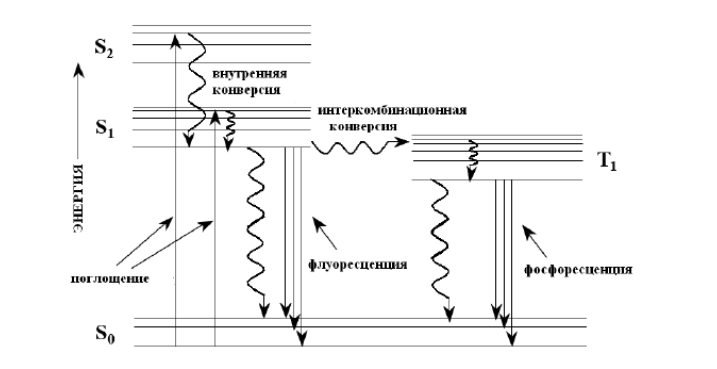
\includegraphics [scale=0.6]{Images/Яблонский.png}}
        \caption{Диаграмма Яблонского.}
    \end{figure}

На этой диаграмме буквами S обозначены синглетные состояния молекулы. Суммарный спин S всех электронов молекулы в таком состоянии равен 0, мультиплетность $М = 2S+1 = 1$. Если суммарный спин молекулы S = 1, то мультиплетность $М = 2S+1 = 3$, и
молекула находится в триплетном состоянии ($T_1,\; T_2$ и т.д.). Это означает, что молекула может
находиться в одном из трех состояний, вырожденных по энергии, и отличающихся друг от друга проекцией спина.
При поглощении света молекула
переходит на один из колебательных подуровней возбужденного электронного состояния. При сохранении мультиплетности возбужденное состояние будет синглетным.
Если возбуждаемый электрон меняет направление спина, возбужденное состояние будет триплетным. Таким образом, одному основному состоянию соответствует набор разных возбужденных состояний — синглетных и триплетных.

Излучательный переход между двумя состояниями одинаковой мультиплетности
называется \textbf{флуоресценцией}, разной мультиплетности — \textbf{фосфоресценцией}.
\subsection{Основные законы флуоресценции}
\begin{wrapfigure}{r}{0.25\textwidth}
    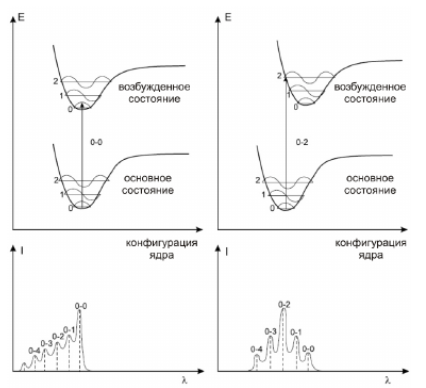
\includegraphics[width=\linewidth]{Images/Франк-Кондон.png}
    \caption{Принцип Франка-Кондона.}
\end{wrapfigure}\
\par \textbf{Закон Стокса:}
В многоатомных молекулах спектр испускания сдвинут относительно спектра
возбуждения в длинноволновую область. Это связано с протеканием процессов
релаксации с верхних подуровней и расщеплением нижнего уровня. Сдвиг между
положением максимумов спектра поглощения и флуоресценции называется \textbf{стоксовым
сдвигом}.

\textbf{Правило Левшина:} Спектры
испускания и возбуждения флуоресценции, как правило, зеркально-симметричны относительно прямой, проходящей через точку их пересечения перпендикулярно оси длин волн. Оно обусловлено сходством распределения колебательных подуровней по энергиям у основного и возбужденного состояний. 

\textbf{Принцип Франка-Кондона:} Электронный переход с излучением светового кванта можно представить вертикальной
линией, соединяющей различные поверхности
потенциальной энергии, причем наиболее вероятным окажется переход на тот колебательный уровень, который имеет то же значение межъядерного расстояния в точке поворота при колебаниях, поскольку вероятность обнаружить молекулу в этих точках выше.

\textbf{Правило Каши:} Излучение фотона (флуоресценция и фосфоресценция) происходит только с низшего возбужденного электронного состояния молекулы. 

\textbf{Правило Вавилова:} Квантовый выход ($\phi = \frac{n_F}{n_a}$) не зависит от длины волны возбуждения, если выполняется закон Стокса, т.е. если длина волны возбуждающего света меньше длины волны флуоресценции.

\subsection{Фотометрический метод анализа концентраций веществ}\
\par Фотометрический метод анализа концентраций веществ основан на том, что каждое
вещество поглощает излучение только с характерными для него длинами волн.
Для истинных растворов поглощение света проявляется в ослаблении светового
потока после прохождения через объект, что выражается законом Бугера-Ламберта-Бэра:

\begin{equation}
    I = I_010^{-\varepsilon Cl} \approx I_0e^{-2,3\varepsilon Cl}
\end{equation}

Для количественного описания способности вещества поглощать излучение обычно
используются два параметра – пропускание ($T$) и оптическая плотность ($D$):

\begin{equation}
    D = lg \frac{I_0}{I} = -lgT
\end{equation}
\begin{equation}
    D = \varepsilon Cl
\end{equation}

Для спектров флуоресценции часто
оказывается, что интенсивность флуоресценции пропорциональна концентрации лишь в ограниченном диапазоне оптических плотностей. Из-за поглощения, вследствие закона Бугера-Ламберта-Бера ($l = 1\;$см),
интенсивность света в центре кюветы $I$ меньше интенсивности света, падающего на кювету $I_0$: $I = I_0 10^{-D}$. Поскольку интенсивность флуоресценции пропорциональна интенсивности падающего света, то кажущийся выход флуоресценции будет ниже, чем для бесконечно разбавленного раствора. Эта особенность называется эффектом внутреннего
фильтра.

Допустим, что образец имеет значительную оптическую плотность как при длине
волны возбуждения, так и при длине волны испускания: $D_{\text{возб}}$ и $D_{\text{исп}}$. 
Исправленная интенсивность флуоресценции при этом приблизительно равна:
\begin{equation}
    F_{\text{испр}} = F_{\text{набл}} 10^{(D_{\text{возб}} + D_{\text{исп}})/2}
\end{equation}
\subsection{Тушение флуоресценции}\
\par Тушением называют любые процессы, приводящие к уменьшению интенсивности флуоресценции данного вещества, как например: реакции в возбуждённом состоянии, перенос энергии, образование комплексов или столкновение с молекулой-гасителем. В данной работе выделяют два типа процесса тушения — динамическое и статическое, в ходе которых флуорофор возвращается в основное состояние без излучения фотона. Первое из них связано со столкновениями между флуорофором и гасителем, эта реакция описывается следующими уравнениями:
\begin{equation}
    M^{*} + Q \xrightarrow{} M + Q;   w = K_{q}[M^{*}][Q]
\end{equation}
\par Уравнение Штерна-Фольмера:
\begin{equation}
    \frac{F_{0}}{F} = 1 + K_{q} \tau [Q] = K_{din} [Q]
\end{equation}
\par где М* и М – флуорофор в возбужденном и невозбужденном состоянии, Q – гаситель, w – скорость бимолекулярной реакции, $K_{q}$ – бимолекулярная константа скорости тушения, $F_{0}$, F – интенсивность флуоресценции в отсутствие и в присутствии гасителя соответственно, $\tau$ – время затухания флуоресценции в отсутствии гасителя, [Q] –
концентрация гасителя, $K_{din}$ = $K_{q}$ $\tau$ – штерн-фольмеровская константа тушения.
\par Частота столкновений флуорофора с гасителем выражается как:
\begin{equation}
    Z = K_{0}[Q] = 4 \pi RDN[Q]
\end{equation}
\par где $K_{0}$ – диффузионно-контролируемая (скорость реакции лимитируется сближением частиц
в результате диффузии) бимолекулярная константа скорости, вычисленная
по уравнению Смолуховского:
R – радиус столкновения (обычно за него принимается сумма радиусов молекул
флуорофора и гасителя), D – сумма коэффициентов диффузии флуорофора и
гасителя, N – число Авогадро.
\par Из следующей связи будет легко оценивать эффективность тушения $w$:
\begin{equation}
    K_{q}= K_{q}w
\end{equation}
\par В данной работе гасителями выступают ионы иода, они, как и бром увеличивают константу интеркомбинационной конверсии в триплетное состояние из-за спин-орбитального взаимодействия, возбуждённого в синглетном состоянии флуорофора и галогена. Время жизни в триплетном состоянии довольно продолжительно, поэтому другие процессы успевают тушить флуорофор.

\par Статическое тушение происходит из-за образования комплекса MQ в основном состоянии, и при поглощении света этот комплекс медленно возвращается в исходное состояние без испускания фотона. Данная реакция описывается следующими уравнениями:
\begin{equation}
    M + Q \xrightarrow{} MQ;   w = K_{q}[M][Q]
\end{equation}
\begin{equation}
    K_{stat} = \frac{[MQ]}{[M][Q]}
\end{equation}
\begin{equation}
    \frac{F_{0}}{F} = 1 + K_{stat}[Q]
\end{equation}
\subsection{Исследование флуоресценции белков}\
\par Явление флуоресценции широко используется в биологических исследованиях, в особенности это связано с изучением белков, содержащих в себе некоторые аминокислоты: триптофан, фенилаланин и тирозин, — которые поглощают в ультрафиолетовой области.
\par Так же существуют молекулы флуоресцентных зондов, которые способны нековалентно связываться с компонентами клетки, например жирными кислотами в мембране. В случае ковалентного пришивания флуорофора к мишени говорят о присоединении метки.
\par Возвращаясь к белкам, беззондовые исследования на практике проводят с белками, содержащими триптофан и тирозин, которые имеют достаточно большой квантовый выход для получения хорошего сигнала флуоресценции. При использовании источника излучения с длинной волны 280 нм обе аминокислоты будут возбуждены, а при 295-305 нм возбуждается преимущественно триптофан. Свойства этих аминокислот позволяют изучать процесс сворачивания белка. В нативном состоянии аминокислоты скрыты внутри белка, то есть имеют гидрофобное окружение и высокий квантовый выход. При денатурации аминокислоты окружены гидрофильной средой, в которой интенсивность флуоресценции заметно падает. Так как денатурация происходит при повышении температуры, то очень важно достигать равновесного состояния при каждом измерении. 
\section{Описание установки}\
\par В работе используется спектрофлуориметр Avantes.
Принцип его работы заключается в следующем: источник (дейтериево-галогеновая лампа) излучает в ультрафиолетовой области, свет попадает на первичный фильтр возбуждения (монохроматор), где осуществляется подбор волн требуемого интервала — остальные блокируются. Уже отобранное излучение проходит через пробу, находящуюся в кювете. После, излучение, испускаемое в ходе флуоресценции попадает на фотодетектор, который преобразует его в электричество.
\begin{figure}[!htb] 
        \minipage{0.45\textwidth}
            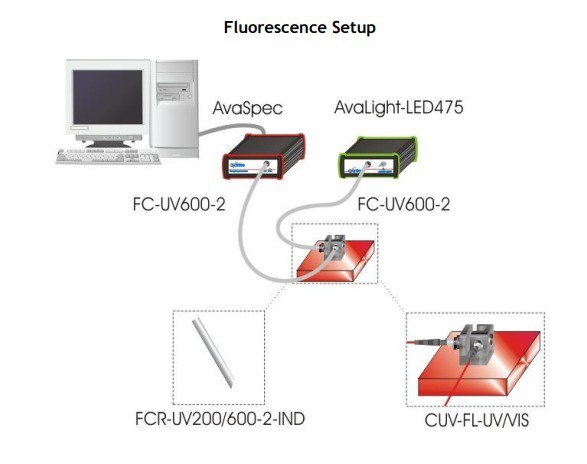
\includegraphics[width=\linewidth]{Images/схема устройства.png}
            \caption{Схема внешнего устройства спектрофлуориметра Avantes.}
        \endminipage\hfill
        \minipage{0.55\textwidth}
             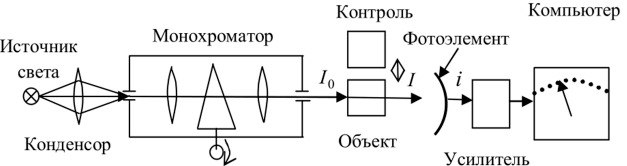
\includegraphics[width=\linewidth]{Images/спектрофотометр.png}
              \caption{Принципиальная схема внутреннего устройства спектрофотометра.}
        \endminipage
    \end{figure}

\section{Результаты и обсуждение}
\subsection{Исследование зависимости спектров поглощения и флуоресценции растворов родамина 6G от концентрации}\
\par Для следующих опытов необходимо подготовить линейку растворов родамина с разной концентрацией ($2 \cdot 10^{-4}, 10^{-4}, 2 \cdot 10^{-5}, 10^{-5}, 2 \cdot 10^{-6}$ M) из стокового $2 \cdot 10^{-4}$ M раствора. Затем снимаем спектры поглощения для каждой концентрации на спектрофотометре Schimadzu UV-1800 (диапазон длин волн от 200 до 800 нм). И так же регистрируем спектр флуоресценции на спектрофотометре Avantes (время измерения - 500 мс, число усреднений - 10, источник излучения - диод(LED)).

\begin{figure}[h!]
    \centering{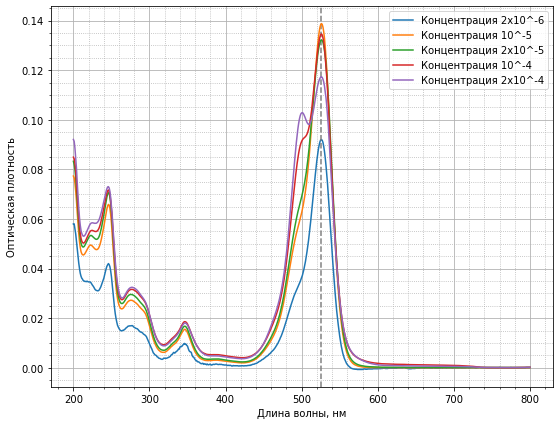
\includegraphics [scale=0.6]{Images/шимадзу.png}}
    \caption{Спектр поглощения растворов родамина со спектрофотометра Schimadzu UV-1800.}
\end{figure}
\par Значения оптической плотности нормировались по концентрации и ширине кюветы для каждого из спектров. Для всех концентраций максимум поглощения приходится на 526 нм, что немного отличается от табличных значений (535 нм). С ростом концентрации оптическая плотность растёт (для 1-2 образцов наименьших концентраций), однако можно предположить, что начиная с достаточно высокой концентрации происходит образование димеров, из-за чего на спектре возникает дополнительный горб (3-4 образец), а а у 5 образца заметен отчётливый второй пик. При этом уменьшается значение для основного пика поглощения родамина, так как уменьшается его концентрация.
\par Из константы реакции диссоциации ($K_{дисс} = 5 \cdot 10^{-4}$ М) можем оценить равновесную концентрацию димеров родамина, которые образуются в наших образцах. Так для стокового раствора концентрация димеров составляет $2 \cdot 10^{-5}$ М, что лишь на порядок отличается от концентрации мономеров. Данный эффект больше всего отражается на форме спектров для образцов 3-5 с наибольшими концентрациями.
\begin{figure}[h!]
    \centering{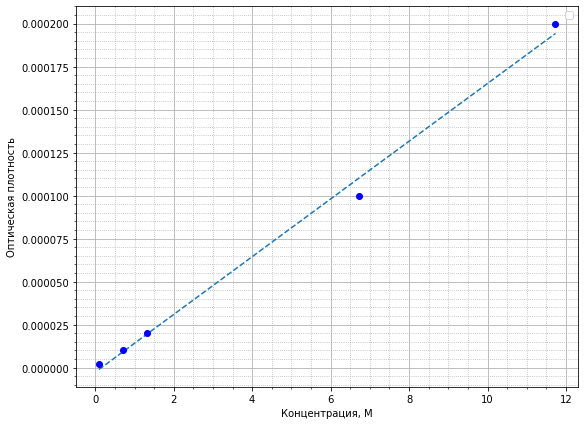
\includegraphics [scale=0.6]{Images/БЛБ.png}}
    \caption{График зависимости оптической плотности от концентрации образца родамина.}
\end{figure}
\par Проверим, выполняется ли закон Бугера-Ламберта-Бера для достаточно больших концентраций стокового раствора родамина и его первых разведений. На графике (рис. 6) представлена линейная зависимость оптической плотности от концентрации, что соотносится с формулой закона. Можно предположить, что для концентраций, использующихся в нашем опыте (до $2 \cdot 10^{-4}$ М) закон Бугера-Ламберта-Бера выполняется.
\begin{figure}[h!]
    \centering{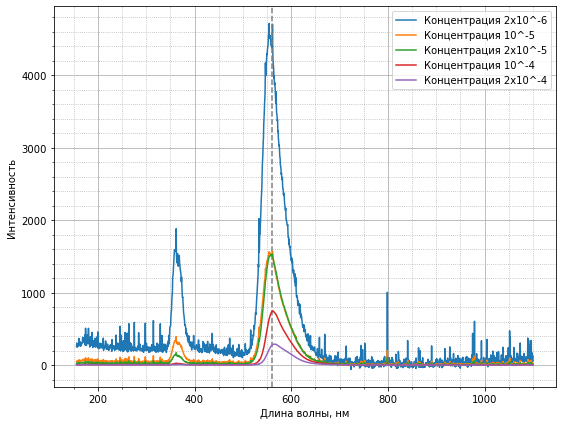
\includegraphics [scale=0.6]{Images/флуориметр.png}}
    \caption{Спектр возбуждения и испускания родамина со спектрофотометра Avantes.}
\end{figure}
\par Теперь рассмотрим данные флуоресценции со спектрофотометра Avantes. На спектре (рис. 7) чётко видны первые пики в районе 365 нм, что отвечает возбуждающему излучению диода. Самый крупный пик немного отличается у образцов, но в среднем находится в районе 560 нм - это максимум испускания в процессе флуоресценции. Необходимо отметить, что спектр сдвинулся в более длинноволновую область относительно спектра поглощения, что соответствует закону Стокса. После нормировки графиков по концентрациям видно, что интенсивность флуоресценции падает с ростом концентрации, что объясняется эффектом фнутреннего фильтра и образованием димеров.
\subsection{Исследование деполяризации флуоресценции эозина (в присутствии БСА)}

\begin{enumerate}
    \item Проведём регистрацию спектров флуоресценции для шести растворов с различной вязкостью. Для этого приготовим растворы со следующими соотношениями рабочих растворов ((а) - $0,1 * PBS$ буферный раствор с pH $\approx 7,4$; (б) - $30 \%$ раствор сахарозы в $0,1 * PBS$ буферном растворе с pH $\approx 7,4$):

    \begin{table}[h!]
    \centering
    \caption{Соотношения растворов первой серии экспериментов}
    \begin{tabular}{|l|l|l|l|l|l|l|}
    \hline
    а, мкл & 100 & 200 & 300 & 400 & 500 & 0 \\ \hline
    б, мкл & 500 & 400 & 300 & 200 & 100 & 600 \\ \hline
    \end{tabular}
    \end{table}

    \item Спектры регистрируются в режиме Absolute Irradiance Mode для горизонтального и вертикального поляризаторов, установленных у стенки кюветы, обращенной к детектору. Пример таких снятых спектров представлены на Рис.. 
    \begin{figure}[h!]
        \caption{Спектры флуоресценции для раствора без добавления сахарозы: 4.1.1 - с горизонтальным фильтром, 4.1.2 - с вертикальным.}
	\centering{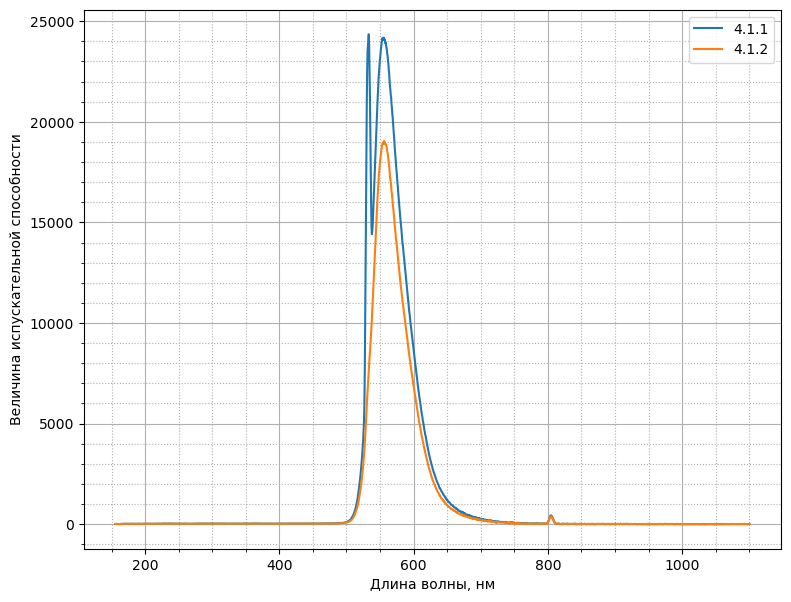
\includegraphics [scale=0.6]{Images/Фото 1.png}}
    \end{figure}

    \item Для данной серии проведём вычисления поляризации по формуле:
    \begin{equation}
        P = \frac{F_{VV} - F_{VH}}{F_{VV} + F_{VH}}
    \end{equation}

    \begin{table}[h!]
    \centering
    \caption{Поляризация растворов первой серии экспериментов}
    \begin{tabular}{|l|l|l|l|l|l|l|}
    \hline
    P & -0,126 & -0,117 & -0,163 & -0,086 & -0,099 & -0,119 \\ \hline
    Вязкость, $10^{-3}$ Па $\cdot$ с & 2,12 & 1,79 & 1,53 & 1,34 & 1,15 & 2,855 \\ \hline
    \end{tabular}
    \end{table}
    \item Проведём аналогичную регистрацию спектров флуоресценции для пяти растворов с различной вязкостью и добавлением БСА. Для этого приготовим растворы со следующими соотношениями рабочих растворов ((в) - $2\%$ раствор БСА в $0,1 * PBS$ буферном растворе с pH $\approx 7,4$; (г) - $2\%$ раствор БСА в $30 \%$ раствор сахарозы в $0,1 * PBS$ буферном растворе с pH $\approx 7,4$):
    \begin{table}[h!]
    \centering
    \caption{Соотношения растворов второй серии экспериментов}
    \begin{tabular}{|l|l|l|l|l|l|}
    \hline
    в, мкл & 100 & 200 & 300 & 400 & 500\\ \hline
    г, мкл & 500 & 400 & 300 & 200 & 100\\ \hline
    \end{tabular}
    \end{table}
    \item Приведём так же сравнительный график двух спектров для вертикального и горизонтального фильтров - Рис.. 
    \begin{figure}[h!]
    \caption{Спектры флуоресценции для раствора с добавлением 100 мкл раствора с сахарозой: 4.7.1 - с горизонтальным фильтром, 4.7.2 - с вертикальным.}
    \centering{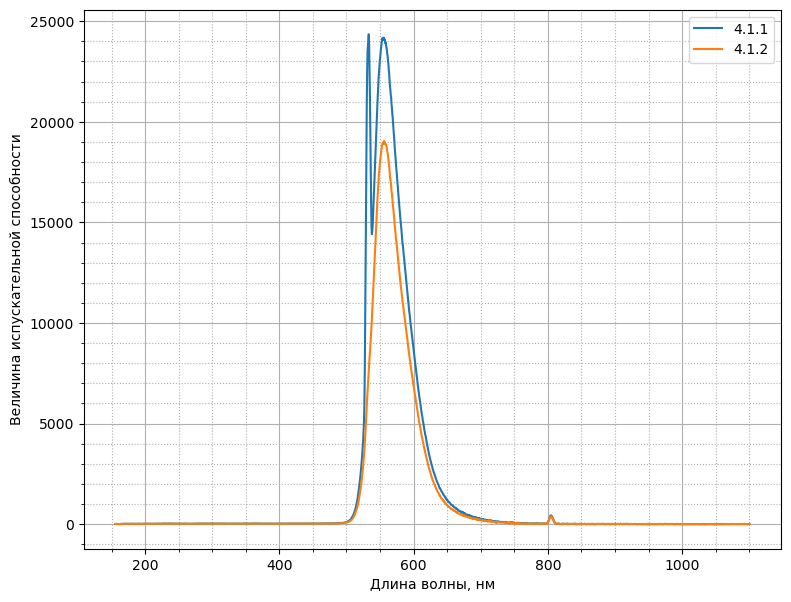
\includegraphics [scale=0.6]{Images/Фото 1.png}}
    \end{figure}
    \item Воспользуемся формулой (14) для аналогичного расчёта величины поляризации:
    \begin{table}[h!]
    \centering
    \caption{Поляризация растворов второй серии экспериментов}
    \begin{tabular}{|l|l|l|l|l|l|}
    \hline
    P & -0,454 & -0,454 & -0,444 & -0,441 & -0,401 \\ \hline
    Вязкость, $10^{-3}$ Па $\cdot$ с & 2,12 & 1,79 & 1,53 & 1,34 & 1,15 \\ \hline
    \end{tabular}
    \end{table}
    \item Для обеих серий воспользуемся зависимостью Левшина-Перрена:
    \begin{equation}
        \frac{1}{P} = \frac{1}{P_0} + \left( \frac{1}{P_0} - \frac{1}{3}\right)\frac{kT\tau_0}{V\eta}
    \end{equation}
    Построим соответствующие прямые и найдём необходимые коэффициенты с помощью МНК:
    \begin{figure}[!htb]
                \minipage{0.5\textwidth}
                 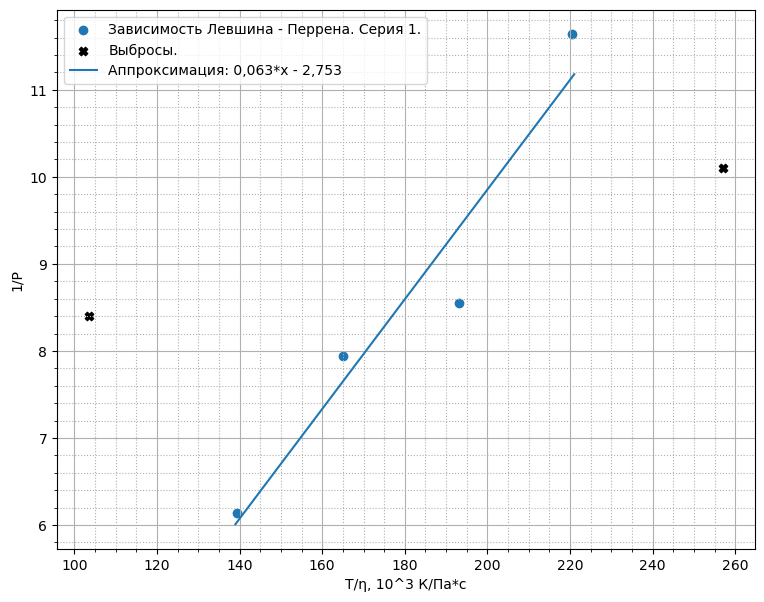
\includegraphics[width=\linewidth]{Images/Фото 3.png}
                 \caption{Первая серия измерений.}
                  \endminipage\hfill
                \minipage{0.5\textwidth}
                 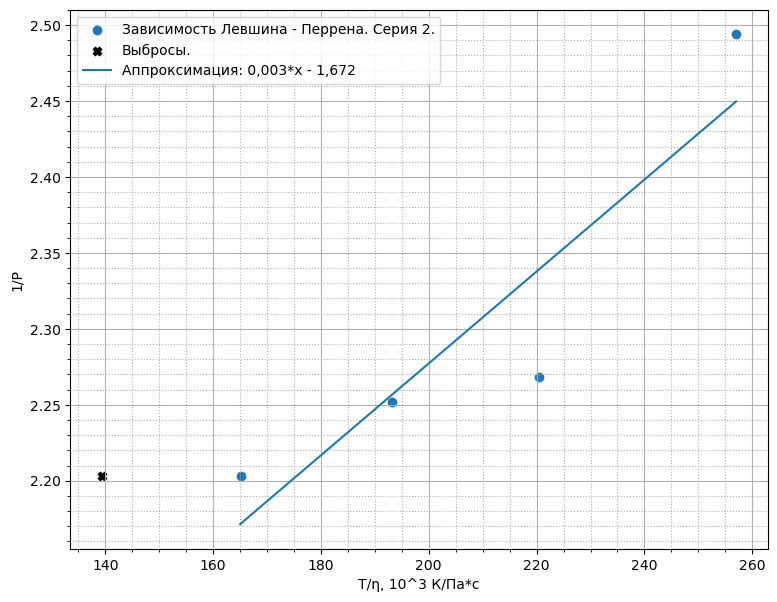
\includegraphics[width=\linewidth]{Images/Фото 4.png}
                 \caption{Вторая серия измерений.}
                  \endminipage
              \end{figure}
    \item Используя зависимость (15), определим следующие параметры:
    \begin{table}[h!]
    \centering
    \caption{Параметры, полученные из двух серий}
    \begin{tabular}{|l|l|l|l|}
    \hline
     & V, $\text{м}^3$ & $P_0$ & a, $10^{-10} \cdot$ м \\ \hline
     Первая серия& 8,78 $\cdot 10^{-30}$ & 0,363 & 2,06 \\ \hline
     Вторая серия& 8,00 $\cdot 10^{-27}$  & 0,598 & 28,29 \\ \hline
    \end{tabular}
    \end{table}

    \item Таким образом, в первой серии экспериментов определялся объём и размер молекулы эозина, а во второй серии - комплекса эозина и БСА. Результаты приведены в Таблице 5. Сравнивая затем полученные данные с литературными источниками, можно придти к выводу, что для эозина значения отличаются примерно в пять раз, а для БСА проходят по нижней границе размеров данного белка.

    \item Последним пунктом нас просили сравнить интенсивности флуоресценции чистого эозина и комплекса эозина с БСА. Рис..
    \begin{figure}[h!]
    \caption{Сравнение спектров из разных серий для растворов с равным соотношением сахарозы}
    \centering{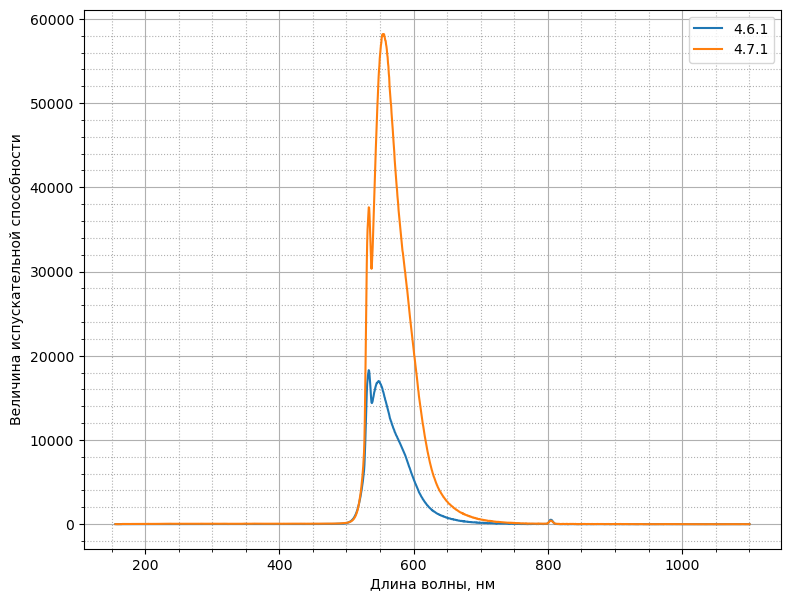
\includegraphics [scale=0.5]{Images/Фото 5.png}}
    \end{figure}
    \item Видно, что интенсивности двух серий сильно отличаются друг от друга. Связано это, вероятно, с тем, что БСА и эозин при данном pH отрицательно заряженные молекулы и тушение флуоресценции не происходит ни динамическим, ни статическим образом.  
\end{enumerate}
    \section{Выводы}
    \begin{itemize}
        \item В первой части работы удалось зарегистрировать спектры поглощения, возбуждения и испускания растворов родамина разной концентрации. Отмечены характерные особенности: увеличение максимума поглощения с ростом концентрации, появление дополнительного пика поглощения и уменьшение основного из-за образования димеров родамина, уменьшение интенсивности флуоресценции в следствии эффекта внутреннего фильтра, смещение спектра флуоресценции в длинноволновую область относительно спектра поглощения (Стоксов сдвиг).
        \item Для серии образцов родамина концентрации от $2 \cdot 10^{-4}$ М до $2 \cdot 10^{-6}$ M была показана применимость закона Бугера-Ламберта-Бера на основе линейной зависимости экспериментальных значений оптической плотности от концентраций.
        \item В последующих частях работы изучался вопрос деполяризации флуоресценции поляризованного света растворами эозина без и с добавлением БСА. Был проведен анализ зависимости Левшина-Перрена и оценка размеров молекул, вызывающих флуоресценцию.
    \end{itemize}
    \section{Список литературы}
    \begin{enumerate}
        \item Лакович Д. Основы флуоресцентной спектроскопии. М.: Мир 1986
        \item Слюсарева Е.А.; ФОТОНИКА ФЛУОРОНОВЫХ КРАСИТЕЛЕЙ В ГОМОГЕННЫХ И ГЕТЕРОГЕННЫХ БИОПОЛИМЕРНЫХ СРЕДАХ; Красноярск, 2014.
        \item Khorolskyi, O.V.; Malomuzh, N.P. Macromolecular sizes of serum albumins in its aqueous solutions. AIMS Biophys. 2020, 7, 219–235.
        \item David R. Lide; CRC Handbook of Chemistry and Physics; CRC Press 2003-2004
        \item https://pubchem.ncbi.nlm.nih.gov/compound/Rhodamine-6G#section=Spectral-Information
    \end{enumerate}
\end{document}
